\subsection{Automating state transformer generation}

\ShowTOC[currentsubsection]

\begin{frame}[fragile]{Recovering app. state with transformers}%{A Sub-title is optional}
\begin{itemize}
\item Transformer logic depends on state of object
\item Used to repair application state, for instance fix a memory leak
% \end{frame}
% 
% \begin{frame}[fragile]{Fixing memory leaks}%{A Sub-title is optional}
\begin{itemize}
\item Fix code so that application does not leak memory
\item Repair data at update time to remove past leak (in a subset of
objects)
  \begin{itemize}
  \item \begin{verbatim}
if leaky-object(o):
  o.field = null
\end{verbatim}
  \item \begin{verbatim}
if leaky-object-in-collection(c, o):
  c.remove(o)
\end{verbatim}
  \end{itemize}
\end{itemize}
\end{itemize}
\end{frame}

\begin{frame}{Eclipse Diff Leak}%{A Sub-title is optional}
\begin{center}
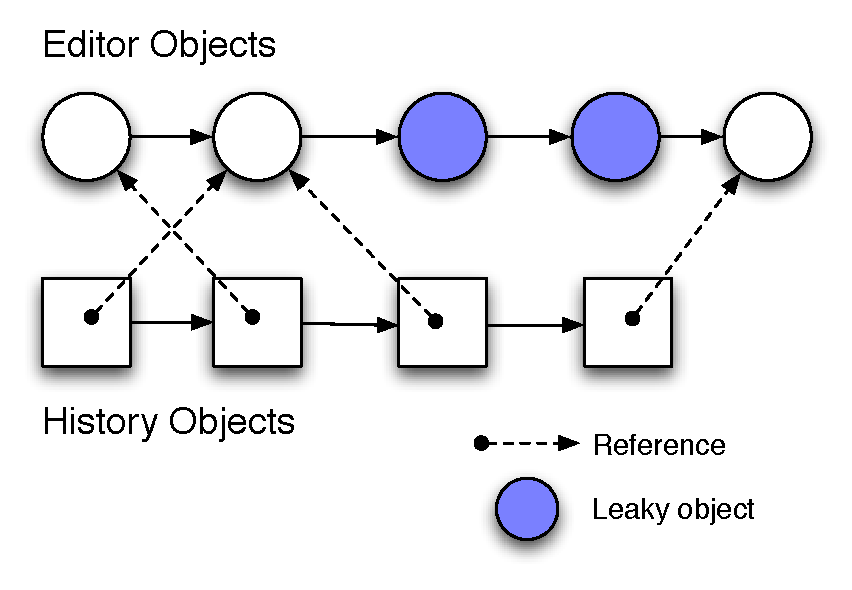
\includegraphics[scale=0.75]{images/eclipse-diff-leak}
\end{center}
\end{frame}

\begin{frame}[fragile]{Eclipse Diff Leak (State transformer)}%{A Sub-title is optional}
\begin{lstlisting}[frame=single]
public static void jvolveObject(NavigationHistory to) {
  // set all refcounts to 0
  for (Editor e : to.editors)
    e.refcount = 0;

  // recompute refcounts
  for (History h : to.history)
    if (h.editor != null)
      h.editor.refcount++;

  // free leaky objects
  for (Editor e : to.editors)
    if (e.refcount == 0)
      nh.editors.remove(e);
}
\end{lstlisting}
\end{frame}

\begin{frame}[fragile]{Automatically generating fixes}%{A Sub-title is optional}
\begin{center}
\begin{minipage}{0.55\textwidth}
\begin{lstlisting}[frame=single]
  class Foo {
    void bar() {
      ...
      if (...) {
        ...
+       this.field = null;
        ...
      }
    }
  }
  \end{lstlisting}
\end{minipage}
\end{center}
\begin{itemize}
\item Identify leaky objects from heap state, at update time?
\item Dynamic analysis to discover predicate that identifies leaky objects
\item Not just leaks, can be used to generate the correct state transformer
\end{itemize}
\end{frame}

\begin{frame}[fragile]{Azureus patch}%{A Sub-title is optional}
\begin{itemize}
\item Adds a new field {\tt BaseMdiEntry.isExpanded}
\item Default transformer would set this field to {\tt false}
\item Instead, we discover the following property
% this.iconBarEnabler.visible == this.sidebar.visible
\begin{lstlisting}[numbers=none]
this.isExpanded == this.soParent.paintListenerHooked
\end{lstlisting}
\end{itemize}
\end{frame}
